\documentclass[11pt,aspectratio=169]{beamer}
\usetheme{Copenhagen}

\AtBeginSection[]{
  \begin{frame}
  \vfill
  \centering
  \begin{beamercolorbox}[sep=8pt,center,shadow=true,rounded=true]{title}
    \usebeamerfont{title}\insertsectionhead\par%
  \end{beamercolorbox}
  \vfill
  \end{frame}
}

\usepackage{amsmath}
\usepackage{amssymb}
\usepackage{bm}
\usepackage{amsthm}
\usepackage{enumerate}
\usepackage{graphicx}
\usepackage{psfrag}
\usepackage{color}
\usepackage{url}
\usepackage{listings}
\usepackage{xcolor}
\usepackage{tikz}
% \usetikzlibrary{positioning}
% \tikzset{main node/.style={circle,fill=gray!20,draw,minimum size=.5cm,inner sep=0pt},}

% \definecolor{codegreen}{rgb}{0,0.5,0}
% \definecolor{codewhite}{rgb}{1,1,1}
% \definecolor{codegray}{rgb}{0.5,0.5,0.5}
% \definecolor{codepurple}{rgb}{0.58,0,0.82}
% \definecolor{codeblack}{rgb}{0,0,0}
% \definecolor{codeorange}{rgb}{0.8,0.4,0}

% \lstdefinestyle{mystyle}{
    % backgroundcolor=\color{codewhite},   
    % commentstyle=\color{codegray},
    % keywordstyle=\color{codegreen},
    % numberstyle=\color{codegray},
    % stringstyle=\color{codeorange},
    % basicstyle=\ttfamily ,
    % breakatwhitespace=false,         
    % breaklines=true,                 
    % captionpos=b,                    
    % keepspaces=true,                 
    % numbers=left,                    
    % numbersep=5pt,                  
    % showspaces=false,                
    % showstringspaces=false,
    % showtabs=false,                  
    % tabsize=4
% }
% \lstset{style=mystyle}


% \setlength{\hoffset}{-1in}
% \addtolength{\textwidth}{1.5in}
% \setlength{\voffset}{-1in}
% \addtolength{\textheight}{1.5in}
\newcommand{\be}{\begin{enumerate}}
\newcommand{\ee}{\end{enumerate}}
\newcommand{\BigO}[1]{\ensuremath\mathcal{O}\left(#1\right)}
\newcommand{\il}[1]{\lstinline!#1!}
\newcommand{\norm}[1]{\left|\left|#1\right|\right|}
\newcommand{\abs}[1]{\left|#1\right|}
\newcommand{\parens}[1]{\left(#1\right)}
\newcommand{\bracks}[1]{\left\{#1\right\}}
\newcommand{\sqbracks}[1]{\left[#1\right]}
\newcommand{\vep}{\varepsilon}
\newcommand{\ceiling}[1]{\left\lceil#1\right\rceil}
\newcommand{\R}{\mathbb{R}}
\newcommand{\N}{\mathbb{N}}
\newcommand{\Z}{\mathbb{Z}}
\newcommand{\F}{\mathbb{F}}
\newcommand{\C}{\mathbb{C}}
\newcommand{\A}{\mathcal{A}}
\newcommand{\hilbert}{\mathcal{H}}
\newcommand{\distrib}[2]{\text{#1}\left(#2\right)}
\newcommand{\dd}[2]{\frac{d#1}{d#2}}
\newcommand{\parshal}[2]{\frac{\partial#1}{\partial#2}}
\newcommand{\abracks}[1]{\left< #1\right>}
\newcommand{\nullspace}[1]{\text{null }#1}
\newcommand{\LT}[1]{\mathcal{L}\parens{#1}}
\newcommand{\poly}[2]{\mathcal{P}_{#1}\parens{#2}}
\newcommand{\cont}[3]{\mathcal{C}_{#1}^{#2}\parens{#3}}
\newcommand{\range}[1]{\text{range }#1}
\newcommand{\one}{\mathbbm{1}}

\title{A study on quantifying effective training of DLDMD}
\author{Joseph A.G. Diaz}
\institute{Master of Science in Applied Mathematics\\ 
           with a Concentration in Dynamical Systems,\\
           San Diego State University}
\date{\today}

\begin{document}

    \frame{\titlepage}

    \begin{frame}
        \frametitle{Introduction}

        In the study of dynamical systems a central problem is how to derive models 
        from measured data to facilitate the prediction of future states. The data-driven
        method Dynamic Mode Decomposition and it's extensions offer a compelling avenue
        in the problem of prediction from time-series data.

        The marriage of these methods with Machine Learning and Neural Networks allows for
        the leveraging the power of these tools in the space. 

        If standard metrics of model training are unavailable, 
    
    \end{frame}

    \begin{frame}
        \frametitle{Introduction - Prediction from time-series}
        As it says on the tin, we seek a predictive model for a time series 
        $\bracks{\boldsymbol{y}_j}_{j=1}^{N^T+1}$, which are the measurements of a 
        uniformly sampled unknown dynamical system of the form
        \begin{equation}
            \dd{\boldsymbol{y}}{t} = f\parens{\boldsymbol{y}(t)},\quad \boldsymbol{y}(0) 
            = \boldsymbol{x} \in \mathcal{M} \subseteq \R^{N_s}
        \end{equation}
        One method that can be leveraged for this is via the Koopman Operator 
        $\mathcal{K}$. If we denote $\boldsymbol{\varphi}(t;\boldsymbol{x}) =
        \boldsymbol{y}(t)$ to be the flow map affiliated with the initial condition 
        $\boldsymbol{x}$ and denote $g: \mathcal{M} \to \C$ to be a square integrable 
        observable of the system then, according to \cite{koopman}, there exists a 
        linear representation of the flow map given by $\mathcal{K}$;
        \begin{equation}
            \mathcal{K}^t g(\boldsymbol{x}) = g(\boldsymbol{\varphi}(t; \boldsymbol{x})),
        \end{equation}
    
    \end{frame}

    \begin{frame}
        \frametitle{Introduction - Infinite Dimensional Linear Operator $\mathcal{K}$}
        In order to actually use this new representation, it suffices to find the 
        eigenvalues $\bracks{\lambda_\ell}$, and their affiliated eigenfunctions 
        $\bracks{\boldsymbol{\phi}_\ell}$, of the Koopman Operator such that
        \begin{equation}
            \mathcal{K}^t\boldsymbol{\phi}_\ell = \exp(t\lambda_\ell)\boldsymbol{\phi}
            _\ell \implies g(\boldsymbol{x}) = \sum_{\ell \in \N} a_\ell \boldsymbol{\phi}_
            \ell(\boldsymbol{x}),    
        \end{equation}
        where we can essentially construct a modal decomposition of $g$. From here 
        advancing the dynamics to time $t$ is equivalent to writing
        \begin{equation}
            \mathcal{K}^{t} g(\boldsymbol{x}) = \sum_{\ell \in \N} a_\ell 
            \exp(t\lambda_\ell)\boldsymbol{\phi}_\ell (\boldsymbol{x})
        \end{equation} 
    \end{frame}

    \begin{frame}
        \frametitle{Introduction - DMD and EDMD}
        \begin{equation}
            g(\boldsymbol{x}) = \sum_{\ell = 1}^{N_O} a_\ell \boldsymbol{\psi}_\ell
            (\boldsymbol{x}) 
        \end{equation}
        which is to say that the observable $g$ exists in a $N_O$-dimensional subspace 
        of $L^2(\mathcal{M})$ with basis functions $\bracks{\boldsymbol{\psi}_\ell}_{\ell=1}^{N_O}$, 
        and applying the Koopman operator implies that
        \begin{align} 
            \mathcal{K}^{\delta t} g(\boldsymbol{x}) &= \sum_{\ell = 1}^{N_O} a_\ell 
            \exp(\delta t\lambda_\ell)\boldsymbol{\psi}_\ell (\boldsymbol{x}) \\
            &= \sum_{\ell = 1}^{N_O} \boldsymbol{\psi}_\ell (\boldsymbol{x})
            (\boldsymbol{K}_O^T
            \boldsymbol{a})_\ell + r(\boldsymbol{x};\boldsymbol{K}_O)
        \end{align}
    \end{frame}

    \begin{frame}
        \frametitle{Introduction - Time advancement}
        for discrete time step $\delta t$. $\boldsymbol{K}_O$ is the $N_O\times N_O$ matrix that 
        \begin{equation}
            \boldsymbol{K}_O = \underset{K}{\text{argmin}}\norm{{\bf\Psi}_+ - K{\bf\Psi}_-}_F^2
        \end{equation}
        and $r(\boldsymbol{x}, \boldsymbol{K}_O)$ is a residual that represents the 
        total error due to DMD. If the ansatz that $g$ lives in a finite dimensional space holds, 
        then $r$ is identically 0. We define ${\bf\Psi}_\pm$ to be
        \begin{equation}
            {\bf\Psi}_- = \parens{\Psi_1\ \Psi_2\ \cdots \Psi_{N_T}},\quad {\bf\Psi}_+ = \parens{
            \Psi_2\ \Psi_3\ \cdots \Psi_{N_T+1}} 
        \end{equation}
        where $\bracks{\Psi_j}$ is an observable of the time series of interest 
        $\bracks{\boldsymbol{y}_j}$. What the expression for $\boldsymbol{K}_O$ tells 
        us is that, we are trying to find a one-step mapping from each data point
        to the next. Practically speaking, $\boldsymbol{K}_O$ is found
        %$\boldsymbol{K}_O$ approximates $\mathcal{K}$ for a one-step mapping and is found 
        using a singular value decomposition (SVD), with which we can write
        \begin{equation}
            {\bf\Psi}_- = {\bf U\Sigma W}^{\dagger} \implies \boldsymbol{K}_O = 
            {\bf\Psi}_+{\bf W\Sigma}^{-P}{\bf U}^{\dagger}
        \end{equation}
    \end{frame}

    \begin{frame}
        \frametitle{Introduction - Flow reconstruction}
        Finding the eigenvalues, eigenfunctions, and Koopman modes comes down to an 
        eigen-decomposition of $\boldsymbol{K}_O$,
        \begin{equation}
            \boldsymbol{K}_O = {\bf VTV}^{-1}, 
        \end{equation}
        with $\lambda_\ell = \ln(({\bf T})_{\ell\ell})/\delta t$,
        from which the dynamics can be approximated as 
        \begin{equation}
            y(t;\boldsymbol{x}) \approx \boldsymbol{K}_m\exp(t{\bf\Lambda}){\bf V}^{-1}\boldsymbol{\Psi}(\boldsymbol{x}) 
        \end{equation}
        where $\boldsymbol{\Psi}$ is the representation of the initial condition in terms of the observables, 
        $\boldsymbol{K}_m$ is the $N_S \times N_O$ matrix whose columns are the Koopman modes 
        $\bracks{{\bf k}_\ell}_{\ell=1}^{N_O}$ which solve the initial value problem
        \begin{equation}
            \boldsymbol{x} = \sum_{\ell=1}^{N_O}{\bf k}_\ell\boldsymbol{\phi}(\boldsymbol{x}),
        \end{equation}
        and ${\bf \Lambda}$ is the diagonal matrix whose elements are $\lambda_\ell
        = ({\bf \Lambda})_{\ell\ell}$.
    \end{frame}

    \begin{frame}
        \frametitle{Introduction - Neural Networks}
        Before we move on, a brief digression on Neural Networks (NNs) is appropriate. Ever since
        scientists discovered the relatively simple interaction between neurons and axons in 
        the human brain, they have been enamored with the ability to create a learning computer 
        with the similar ability to become more adept at a task with training and practice. 
        In the same way that art imitates life, the most straight-forward attempts have been 
        to construct artificial neural networks that pantomime the biological ones that we carry 
        around in our heads; and while these pale imitations have not been developed to rival the 
        human brain, they have led to some major achievements in automation. In much the same 
        way that a person is ``trained'' to perform a task by repeating it with feedback and 
        adjusting their performance as they go, an artificial NN uses data, a loss function, and 
        an optimization algorithm to change the state of the NN to one which can better accomplish 
        the task. The loss function and optimizer are to the feedback and behavioral adjustment 
        what the data is to the experience. 
    \end{frame}

    \begin{frame}
        \frametitle{Introduction - Function approximation and regression}
        Say we have a set of training data $d_{tr} = \bracks{(x_j, y_j)}_{j=1}^{N_{tr}}$ 
        and we believe that there is some function $f(x)$ such that 
        \begin{equation}
            y_j = f(x_j) + \vep_j,    
        \end{equation}
        where $\vep_j$ is assumed to be a sample drawn from $\mathcal{N}(0, \bar{\sigma}^2)$. 
        \cite{oreilly, theodoridis}
        Generally $f$ is not known; so we must, using the training data, build an estimator 
        $f_e(x; d_{tr})$ and measure the performance of the estimator by examining the quantity
        \begin{equation}
            \mathbb{E}_{d_{tr}}\sqbracks{\parens{f(x) + \vep - f_e(x;d_{tr})}^2} = 
            \text{bias}_{d_{tr}}^2 + \mathbb{V}(f_e) + \bar{\sigma}^2
        \end{equation}
        where 
        \begin{equation}
            \text{bias}_{d_{tr}} = \mathbb{E}_{d_{tr}}\sqbracks{f_e} - f(x)
        \end{equation}
        and 
        \begin{equation}
            \mathbb{V}(f_e) = \mathbb{E}_{d_{tr}}\sqbracks{\parens{\mathbb{E}_{d_{tr}}
            \sqbracks{f_e} - f_e(x; d_{tr})}^2}
        \end{equation}
        % With this framing, ML methods can be cast as attempts to find an estimator relative to
        % a given training set that balances the competing dilemmas of being too biased or allowing too
        % much variance. From the point of view of non-parametric statistics, we would need to utilize 
        % other techniques \cite{hollander} to determine the bias and variance of any given estimator. 
        For our purposes, 
        we will instead consider how metrics from information theory can be used to assess the change in 
        information as data is fed through a NN and a model is trained.
    \end{frame}

    \begin{frame}
        \frametitle{Introduction - DLDMD}
        The key innovation of 
        \cite{lago} is to use a neural network to come up with the collection of 
        observables on $\bracks{\boldsymbol{y}_j}$ that allow for the best prediction 
        of future system states, we call this method Deep Learning Enhanced DMD (DLDMD). 
        This is implemented by defining an encoder 
        $\mathcal{E}: \R^{N_S} \to \R^{N_O}$ and decoder $\mathcal{D}: \R^{N_O} \to \R^{N_S}$ composed of 
        dense layers such that 
        \begin{equation}
            (\mathcal{D}\circ\mathcal{E})(\boldsymbol{x}) = \boldsymbol{x}
        \end{equation}
        We choose $N_O \geq N_S$ and an appropriate loss function so that 
        $\mathcal{E}$ and $\mathcal{D}$ give a richer space of observables, called the 
        latent space, for EDMD to use when advancing the dynamics. The implementation 
        of NNs for this purpose requires a method of tuning to allow $\mathcal{E}$ and 
        $\mathcal{D}$ to learn the best representations possible. 
    \end{frame}
    
    \begin{frame}
        \frametitle{Introduction - The loss function}
        A natural choice
        considering these constraints is given by
        \begin{equation}
            \mathcal{L} = \alpha_1 \mathcal{L}_{\text{recon}} + \alpha_2 \mathcal{L}
            _{\text{dmd}} + \alpha_3 \mathcal{L}_{\text{pred}} +\alpha_4 
            \norm{\boldsymbol{W}_g}_2 \label{eqn:loss function} 
        \end{equation}
        where 
        \begin{align}
            \mathcal{L}_{\text{recon}} &= \frac{1}{N_T + 1}\sum_{j=1}^{N_T+1}\norm{\boldsymbol{y}_j - 
            (\mathcal{D}\circ\mathcal{E})(\boldsymbol{y}_j)}_2, \\
            \mathcal{L}_{\text{dmd}} &= E_r(\boldsymbol{K}_O), \\
            \mathcal{L}_{\text{pred}} &= \frac{1}{N_T}\sum_{j=1}^{N_T}\norm{\boldsymbol{y}_{j+1} - 
            \mathcal{D}\parens{VT^j V^{-1}\mathcal{E}(\boldsymbol{x})}}_2, \label{eqn:blah}
        \end{align}
        Recall that $N_T$ is the number of measurements in our time-series data after the first.
    \end{frame}

    \begin{frame}
        \frametitle{Introduction - }

    \end{frame}

    \begin{frame}
        \frametitle{Introduction - The Network}
        Example of DLDMD newtork with $N_S = 2,\ N_O = 4,$ and $N_L = 3$ where every
        hidden layer has 16 neurons. The layers in the Figure are 
        labeled, sequentially, left to right: Enc in, Enc 0, Enc 1, Enc 2, Enc out, Dec in, 
        Dec 0, Dec 1, Dec 2, Dec out.
        \begin{figure}
            \centering
            \begin{minipage}{.5\textwidth}
                $$\mathcal{E}$$
                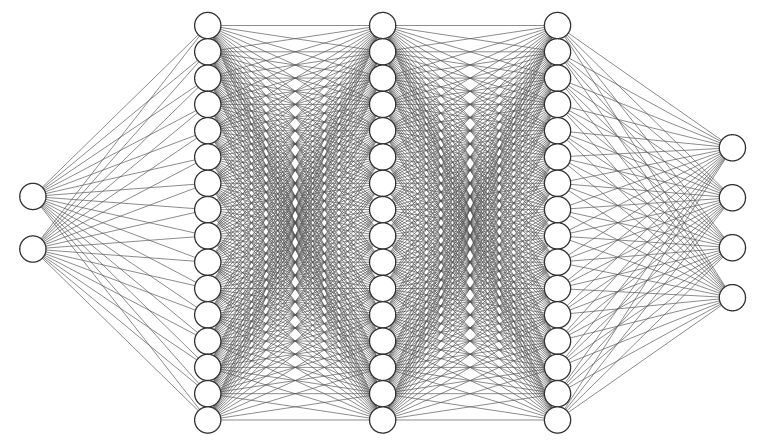
\includegraphics[width=\textwidth]{../Figures/Encoder.png}
            \end{minipage}%
            \begin{minipage}{.5\textwidth}
                $$\mathcal{D}$$
                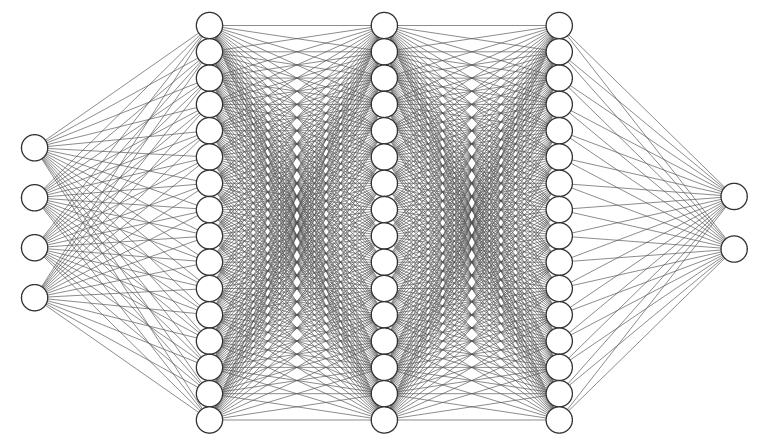
\includegraphics[width=\textwidth]{../Figures/Decoder.png}
            \end{minipage}
        \end{figure}
    \end{frame}

    \begin{frame}
        \frametitle{Kullback-Leibler Divergence - Entropy}
        \begin{figure}
            \centering
            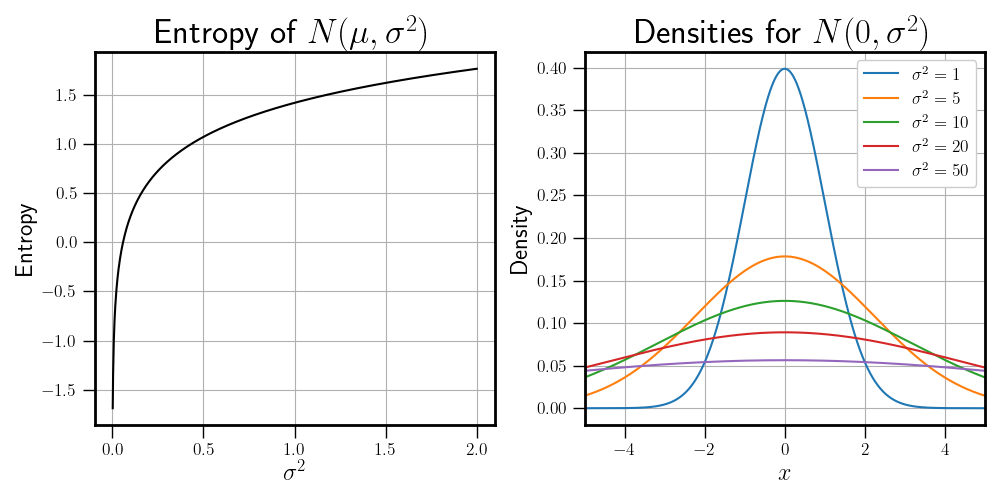
\includegraphics[width=\textwidth]{../Figures/entropy_densities_example.png}
        \end{figure}
    \end{frame}

    \begin{frame}
        \frametitle{Kullback-Leibler Divergence - normal distribution example}
        \begin{figure}
            \centering
            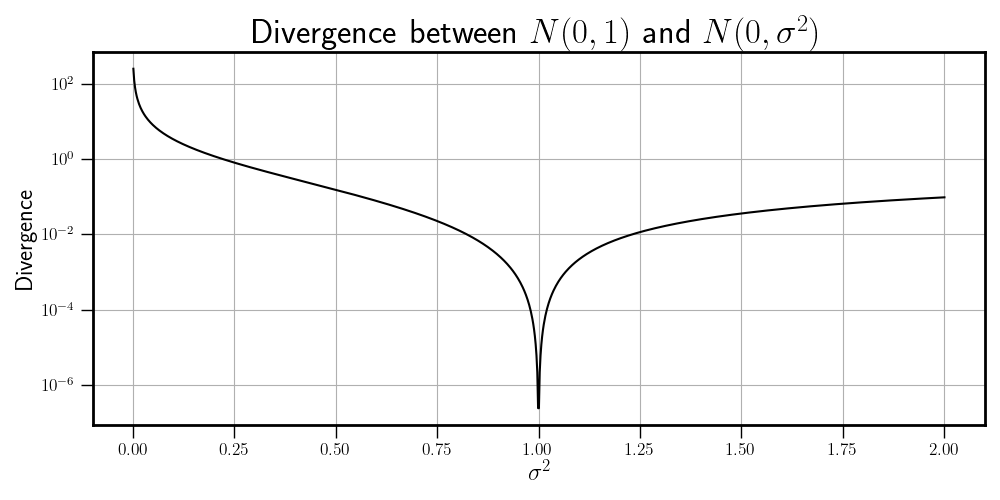
\includegraphics[width=\textwidth]{../Figures/divergence_example.png}
        \end{figure}
    \end{frame}

    \begin{frame}
        \frametitle{Kullback-Leibler Divergence - KDE example}
        \begin{figure}
            \centering
            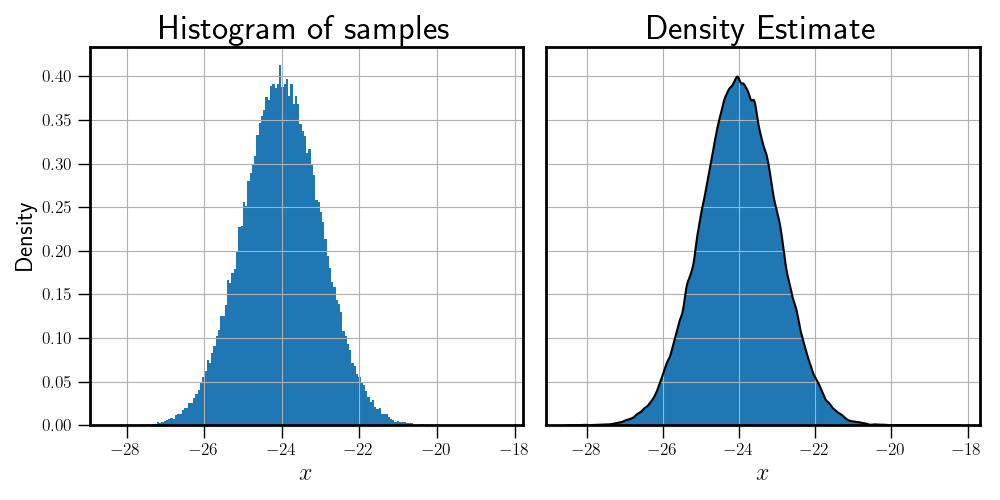
\includegraphics[width=\textwidth]{../Figures/kde_example.png}
        \end{figure}
    \end{frame}

    \begin{frame}
        \frametitle{Kullback-Leibler Divergence - Example fitting}
        \begin{figure}
            \centering
            \includegraphics[width=\textwidth]{"Z:/ML_models/DLDMD-newest/examples/van_der_pol/trained_models/van_der_pol_07_2022-07-17-1837/div_plot_linear_enc_1"}
        \end{figure}
    \end{frame}

    \begin{frame}
        \frametitle{Results - Duffing}
        % $$\ddot{x} + \delta\dot{x} + \alpha x + \beta x^3 = \gamma\cos(\omega t) \to 
        % \begin{cases}
            % & \dot{x} = y \\
            % & \dot{y} = x - x^3  
        % \end{cases}$$
        \begin{figure}
            \centering
            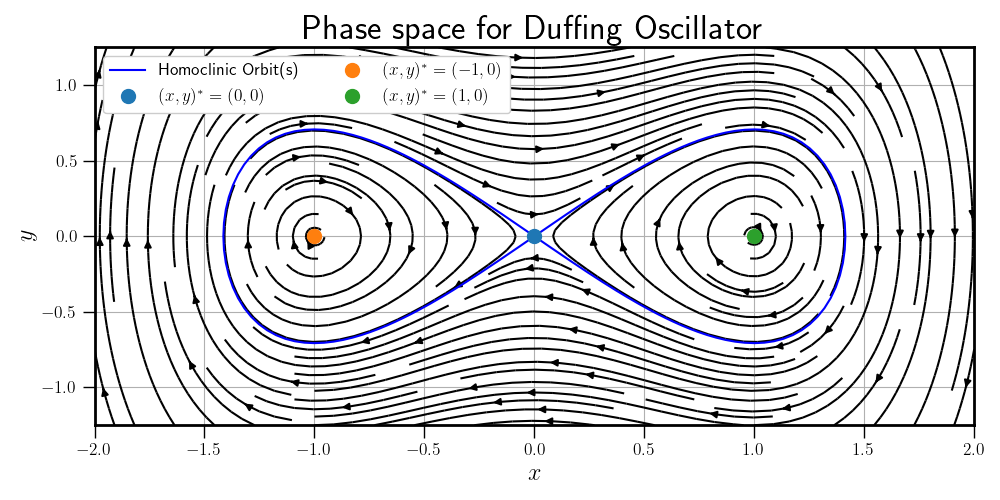
\includegraphics[width=\textwidth]{../Figures/duffing_phase_space.png}
        \end{figure}
    \end{frame}

    \begin{frame}
        \frametitle{Results - Duffing loss curves and phase space}
        \begin{figure}
            \centering
            \begin{minipage}{.5\textwidth}
                \includegraphics[width=\textwidth]{"Z:/ML_models/DLDMD-newest/examples/duffing/loss_plots_square.png"}
            \end{minipage}%
            \begin{minipage}{.5\textwidth}
                \includegraphics[width=\textwidth]{"Z:/ML_models/DLDMD-newest/examples/duffing/experiment_trajectories.png"}
            \end{minipage}
        \end{figure}
    \end{frame}
    
    \begin{frame}
        \frametitle{Results - Duffing linear fit slopes}
        \begin{figure}
            \centering
            \begin{minipage}{.3333\textwidth}
                \includegraphics[width=\textwidth]{"Z:/ML_models/DLDMD-newest/examples/duffing/slope_linear_fit_enc_in_square.png"}
                \includegraphics[width=\textwidth]{"Z:/ML_models/DLDMD-newest/examples/duffing/slope_linear_fit_enc_2_square.png"}
                \includegraphics[width=\textwidth]{"Z:/ML_models/DLDMD-newest/examples/duffing/slope_linear_fit_dec_0_square.png"}
            \end{minipage}%
            \begin{minipage}{.3333\textwidth}
                \includegraphics[width=\textwidth]{"Z:/ML_models/DLDMD-newest/examples/duffing/slope_linear_fit_enc_0_square.png"}
                \includegraphics[width=\textwidth]{"Z:/ML_models/DLDMD-newest/examples/duffing/slope_linear_fit_enc_out_square.png"}
                \includegraphics[width=\textwidth]{"Z:/ML_models/DLDMD-newest/examples/duffing/slope_linear_fit_dec_1_square.png"}
            \end{minipage}%
            \begin{minipage}{.3333\textwidth}
                \includegraphics[width=\textwidth]{"Z:/ML_models/DLDMD-newest/examples/duffing/slope_linear_fit_enc_1_square.png"}
                \includegraphics[width=\textwidth]{"Z:/ML_models/DLDMD-newest/examples/duffing/slope_linear_fit_dec_in_square.png"}
                \includegraphics[width=\textwidth]{"Z:/ML_models/DLDMD-newest/examples/duffing/slope_linear_fit_dec_2_square.png"}
            \end{minipage}
            \includegraphics[width=.3333\textwidth]{"Z:/ML_models/DLDMD-newest/examples/duffing/slope_linear_fit_dec_out_square.png"}
        \end{figure}
    \end{frame}

    \begin{frame}
        \frametitle{Results - Duffing linear fit slope averages and variances}
        \begin{figure}
            \centering
            \includegraphics[width=\textwidth]{"Z:/ML_models/DLDMD-newest/examples/duffing/slope_linear_fit.png"}
        \end{figure}
    \end{frame}

    \begin{frame}
        \frametitle{Results - Duffing notes}

    \end{frame}

    \begin{frame}
        \frametitle{Results - Van der Pol}
        \begin{figure}
            \centering
            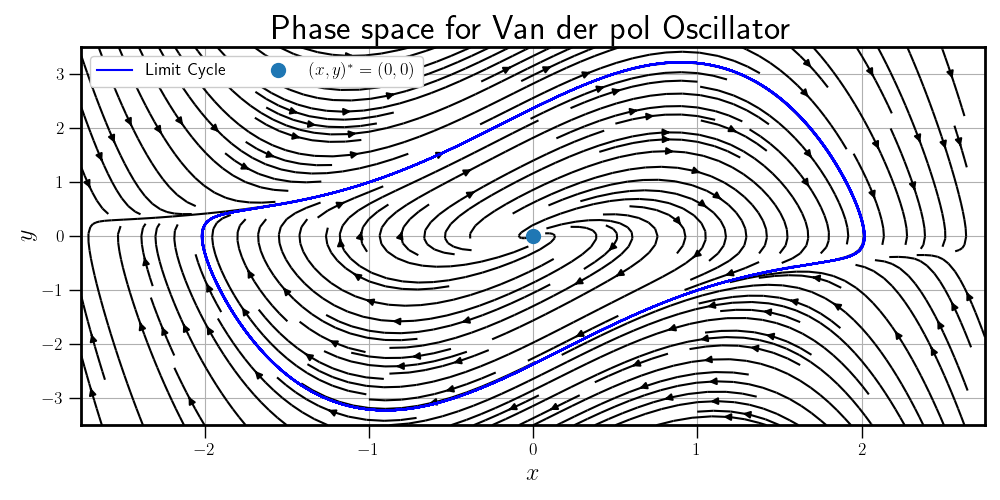
\includegraphics[width=\textwidth]{../Figures/van_der_pol_phase_space.png}
        \end{figure}
    \end{frame}

    \begin{frame}
        \frametitle{Results - Van der Pol loss curves and phase space}
        \begin{figure}
            \centering
            \begin{minipage}{.5\textwidth}
                \includegraphics[width=\textwidth]{"Z:/ML_models/DLDMD-newest/examples/van_der_pol/loss_plots_square.png"}
            \end{minipage}%
            \begin{minipage}{.5\textwidth}
                \includegraphics[width=\textwidth]{"Z:/ML_models/DLDMD-newest/examples/van_der_pol/experiment_trajectories.png"}
            \end{minipage}
        \end{figure}
    \end{frame}

    \begin{frame}
        \frametitle{Results - Van der Pol linear fit slopes} 
        \begin{figure}
            \centering
            \begin{minipage}{.3333\textwidth}
                \includegraphics[width=\textwidth]{"Z:/ML_models/DLDMD-newest/examples/van_der_pol/slope_linear_fit_enc_in_square.png"}
                \includegraphics[width=\textwidth]{"Z:/ML_models/DLDMD-newest/examples/van_der_pol/slope_linear_fit_enc_2_square.png"}
                \includegraphics[width=\textwidth]{"Z:/ML_models/DLDMD-newest/examples/van_der_pol/slope_linear_fit_dec_0_square.png"}
            \end{minipage}%
            \begin{minipage}{.3333\textwidth}
                \includegraphics[width=\textwidth]{"Z:/ML_models/DLDMD-newest/examples/van_der_pol/slope_linear_fit_enc_0_square.png"}
                \includegraphics[width=\textwidth]{"Z:/ML_models/DLDMD-newest/examples/van_der_pol/slope_linear_fit_enc_out_square.png"}
                \includegraphics[width=\textwidth]{"Z:/ML_models/DLDMD-newest/examples/van_der_pol/slope_linear_fit_dec_1_square.png"}
            \end{minipage}%
            \begin{minipage}{.3333\textwidth}
                \includegraphics[width=\textwidth]{"Z:/ML_models/DLDMD-newest/examples/van_der_pol/slope_linear_fit_enc_1_square.png"}
                \includegraphics[width=\textwidth]{"Z:/ML_models/DLDMD-newest/examples/van_der_pol/slope_linear_fit_dec_in_square.png"}
                \includegraphics[width=\textwidth]{"Z:/ML_models/DLDMD-newest/examples/van_der_pol/slope_linear_fit_dec_2_square.png"}
            \end{minipage}
            \includegraphics[width=.3333\textwidth]{"Z:/ML_models/DLDMD-newest/examples/van_der_pol/slope_linear_fit_dec_out_square.png"}
        \end{figure}
    \end{frame}

    \begin{frame}
        \frametitle{Results - Van der Pol linear fit slope averages and variances}
        
        \begin{figure}
            \centering
            \includegraphics[width=\textwidth]{"Z:/ML_models/DLDMD-newest/examples/van_der_pol/slope_linear_fit.png"}
        \end{figure}
    \end{frame}

    \begin{frame}
        \frametitle{Results - Van der Pol notes}

    \end{frame}

    \begin{frame}
        \frametitle{Discussion}

    \end{frame}


    \begin{frame}
        \frametitle{References}
        \bibliographystyle{plain}
        \bibliography{main.bib}
    \end{frame}

    \begin{frame}
        \frametitle{The End!}
        \begin{center}
            \LARGE{Thank you for your time!} \\
            \LARGE{Questions?}
        \end{center}
    \end{frame}
\end{document}